\documentclass[a4paper, 14pt]{article}				% general format

\usepackage[utf8]{inputenc}					% accept different input encodings
\usepackage[russian]{babel}					% multilingual support (T2A)
\usepackage{graphicx}
\usepackage{float}
\usepackage{amsmath}
\usepackage[boxed]{algorithm2e}
\usepackage{url}
\usepackage{fancyvrb}
\usepackage[dvipsnames]{xcolor}

\usepackage{listings}						% typeset source code listings

% Цвета для кода
\definecolor{string}{HTML}{101AF9}			% цвет строк в коде
\definecolor{comment}{HTML}{3F7F5F}		% цвет комментариев в коде
\definecolor{keyword}{HTML}{5F1441}			% цвет ключевых слов в коде
\definecolor{morecomment}{HTML}{8000FF}		% цвет include и других элементов в коде
\definecolor{captiontext}{HTML}{FFFFFF}		% цвет текста заголовка в коде
\definecolor{captionbk}{HTML}{999999}		% цвет фона заголовка в коде
\definecolor{bk}{HTML}{FFFFFF}			% цвет фона в коде
\definecolor{frame}{HTML}{999999}			% цвет рамки в коде

% Настройки отображения кода
\lstset{
	language=C++,						% Язык кода по умолчанию
	% Цвета
	keywordstyle=\color{keyword}\ttfamily\bfseries,
	stringstyle=\color{string}\ttfamily,
	commentstyle=\color{comment}\ttfamily\itshape,
	morecomment=[l][\color{morecomment}]{\#},
	% Настройки отображения
	breaklines=true,					% Перенос длинных строк
	basicstyle=\ttfamily\footnotesize,		% Шрифт для отображения кода
	backgroundcolor=\color{bk},			% Цвет фона кода
	frame=tblr						% draw a frame at all sides of the code block
	rulecolor=\color{frame},				% Цвет рамки
	tabsize=2,						% tab space width
	showstringspaces=false,				% don't mark spaces in strings
	% Настройка отображения номеров строк. Если не нужно, то удалите весь блок
	numbers=left,					% Слева отображаются номера строк
	stepnumber=1,					% Каждую строку нумеровать
	numbersep=5pt,					% Отступ от кода
	numberstyle=\small\color{black},			% Стиль написания номеров строк
	}
% Для настройки заголовка кода
\usepackage{caption}
\DeclareCaptionFont{white}{\color{сaptiontext}}
\DeclareCaptionFormat{listing}{\parbox{\linewidth}{\colorbox{сaptionbk}{\parbox{\linewidth}{#1#2#3}}\vskip-4pt}}
%\captionsetup[lstlisting]{format=listing,labelfont=white,textfont=white}
\renewcommand{\lstlistingname}{Листинг} % Переименование Listings в нужное именование структуры

\author{Певцов Игорь, гр.53501/3}
\title{Отчет по лабораторной работе 6:\\"Набор инструментов для аудита беспроводных сетей AirCrack"\\ по дисциплине\\"Методы и средства защиты информации"}

\begin{document}
\maketitle

\newpage
\tableofcontents{}

\newpage
\section{Цель работы}
Изучить основные возможности пакета AirCrack и принципы взлома WPA/WPA2 PSK и WEP.
\section{Ход работы}


\subsection{Изучение}
\subsubsection{Основные утилиты пакета}
\begin{itemize}
\item airmon-ng - включение и отключение режима мониторинга беспроводных интерфейсов.
\item airodump-ng - программа предназначенная для захвата сырых пакетов протокола 802.11 и особенно подходящая для сбора WEP IVов (Векторов Инициализации) с последующим их использованием в aircrack-ng. Если к вашему компьютеру подсоединен GPS навигатор
то airodump-ng способен отмечать координаты точек на картах

\item aireplay-ng - Основная функция программы заключается в генерации трафика для последующего использования в aircrack-ng для взлома WEP и WPA-PSK ключей.

\item aircrack-ng - Взламывает ключи WEP и WPA (Перебор по словарю).
\end{itemize}

\subsubsection{Утилита airodump}
Опции:
\begin{itemize}
\item{--ivs : Сохранять только отловленные IVы. Короткая форма -i.}
\item{--gpsd : Использовать GPS. Короткая форма -g.}
\item{--write <prefix> : Перфикс файла дампа. Короткая форма -w.}
\item{--beacons : Записывать все маяки в файл дампа. Короткая форма -e.}
\item{--netmask <netmask> : Фильтровать точки по маске. Короткая форма -m.}
\item{--bssid <bssid> : Фильтровать точки по BSSID. Короткая форма -d.}
\item{--encrypt <suite> : Фильтровать точки по типу шифрования. Короткая форма -t}
\item{-a : Фильтровать неасоциированых клиентов}
\item{--channel <channels>: Определить канал. Короткая форма -c.}
\item{--band <abg> :Полоса на которой airodump-ng будет отлавливать пакеты. Короткая форма -b.}
\item{--cswitch <method> : Установить метод переключения каналов. Короткая форма -s. \\
0 : FIFO (по умолчанию)\\
1 : Round Robin\\
2 : Hop on last}
\end{itemize}



\subsection{Запуск режима мониторинга на беспроводном интерфейсе}
Режим мониторинга включается командой
\begin{Verbatim}[frame=single]
airmon-ng start wlan0
\end{Verbatim}

\begin{figure}[h!]
\centering
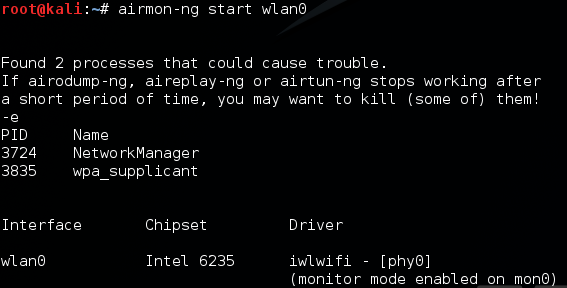
\includegraphics[width=\textwidth]{rsrc/lab6_airmon_start}
\caption{Запуск режима мониторинга на беспроводном интерфейсе wlan0.}
\end{figure}

\subsection{Запуск сбора трафика для получения аутентификационных сообщений}
Сбор трафика запускается командой
\begin{Verbatim}[frame=single]
airdump-ng mon0
\end{Verbatim}

\begin{figure}[h!]
\centering
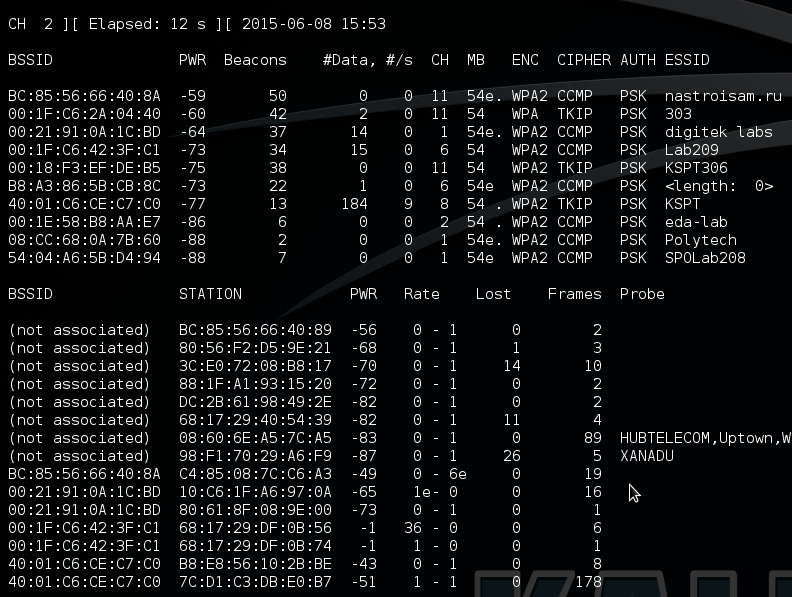
\includegraphics[width=\textwidth]{rsrc/lab6_airodump_start}
\caption{Запуск сбора трафика для получения аутентификационных сообщений.}
\end{figure}

\newpage
Выбираем сеть с BSSID 40:01:C6:CE:C7:C0 и начинаем ее прослушивать(запись в файл airdump, прослушивание 8 канала):
\begin{Verbatim}[frame=single]
airdump-ng mon0 --write airdump --bssid 40:01:C6:CE:C7:C0 -c 8
\end{Verbatim}

\begin{figure}[h!]
\centering
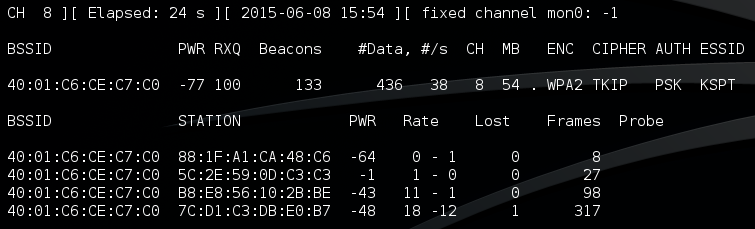
\includegraphics[width=\textwidth]{rsrc/lab6_airodump_bssid}
\caption{Запуск сбора трафика для прослушивания выбранной сети.}
\end{figure}
Видим узлы, подключенные к данной сети. Попробуем провести деаутентификацию одного из узлов c MAC-адресом 7C:D1:C3:DB:E0:B7.

\begin{figure}[h!]
\centering
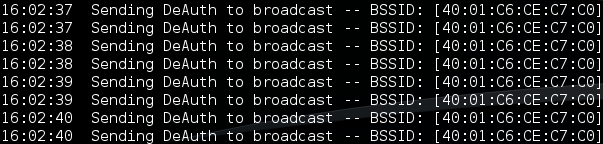
\includegraphics[width=\textwidth]{rsrc/lab6_deauth}
\caption{Процесс деаутентификации.}
\end{figure}
\newpage
Параллельно с этим прослушиваем данную сеть.
\begin{Verbatim}[frame=single]
airdump-ng mon0 --write airdump --bssid 40:01:C6:CE:C7:C0 -c 8
\end{Verbatim}
\begin{figure}[h!]
\centering
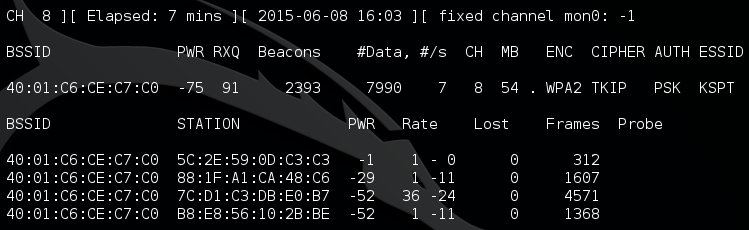
\includegraphics[width=\textwidth]{rsrc/lab6_airodump_bssid_attack}
\caption{Процесс прослушивания сети при деаутентификации. Видно большое количество трафика у хоста c MAC-адресом 7C:D1:C3:DB:E0:B7.}
\end{figure}

\newpage
\subsection{Взлом с использованием словаря паролей}
После длительных тестов мне так и не удалось получить хэндшейк. Тем не менее, чтобы взломать пароль можно воспользоваться командой
\begin{Verbatim}[frame=single]
aircrack-ng airdump-02.cap -w /home/dict.dic
\end{Verbatim}
Где airdump-02.cap - название файла дампа, а dict.dic - название словаря, по которому осуществляется перебор паролей(каждое слово на новой строчке).

Поскольку хэндшейк не был найден, пароль не восстановить
\begin{figure}[h!]
\centering
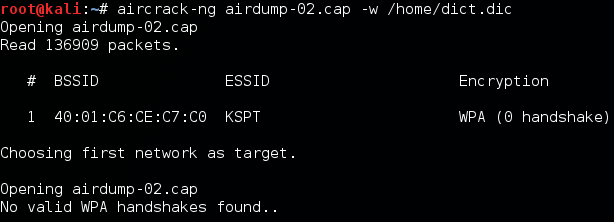
\includegraphics[width=\textwidth]{rsrc/lab6_crack}
\caption{Чтение файла и проверка на наличие хэндшейков. Поскольку хэндшейков нету, взлом не выполняется.}
\end{figure}

\section{Выводы}
В ходе данной работы были изучены основные возможности пакеты Air Crack и принципы взлома WPA/WPA2 PSK. Данный инструмент позволяет прослушивать пакеты, генерировать новые и на основе handshake осуществлять взлом пароля сети. Следует отметить, что пароли, отвечающие минимальным требованиям безопасности не представляется возможном взломать, так как единственный возможный вариант - это перебор. Таким образом, нельзя сказать, что протокол WPA уязвим на данный момент. Протокол WEP является наиболее уязвимым, однако число устройств, использующих его стремится к нулю.
\end{document}